\section{Resultater}
opsummering af m�linger
\\
% impulsrespons
\begin{figure}[h!]
\begin{center}
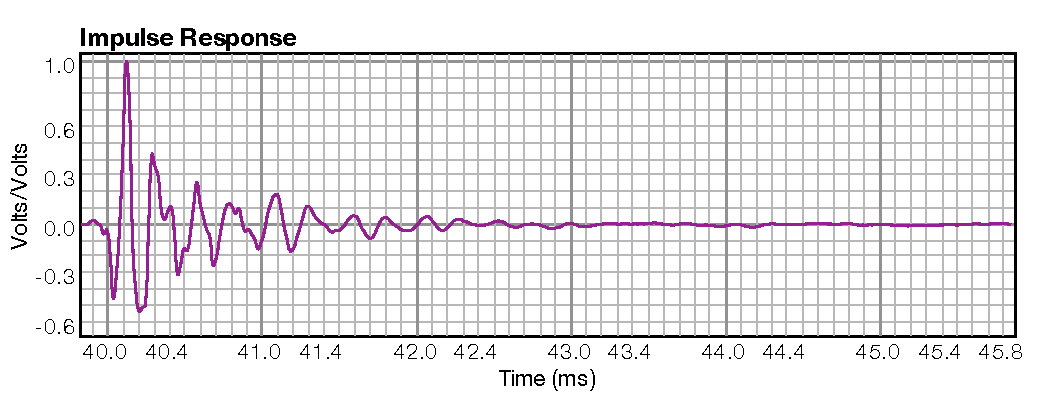
\includegraphics[width=12cm]{impulsrespons.pdf}
\end{center}
\caption{H�jttalerens impulsrespons, on-axis med kabinet}
\label{impuls}
\end{figure}

% alle paa een gang, shell, no+shell
\begin{figure}
\begin{center}
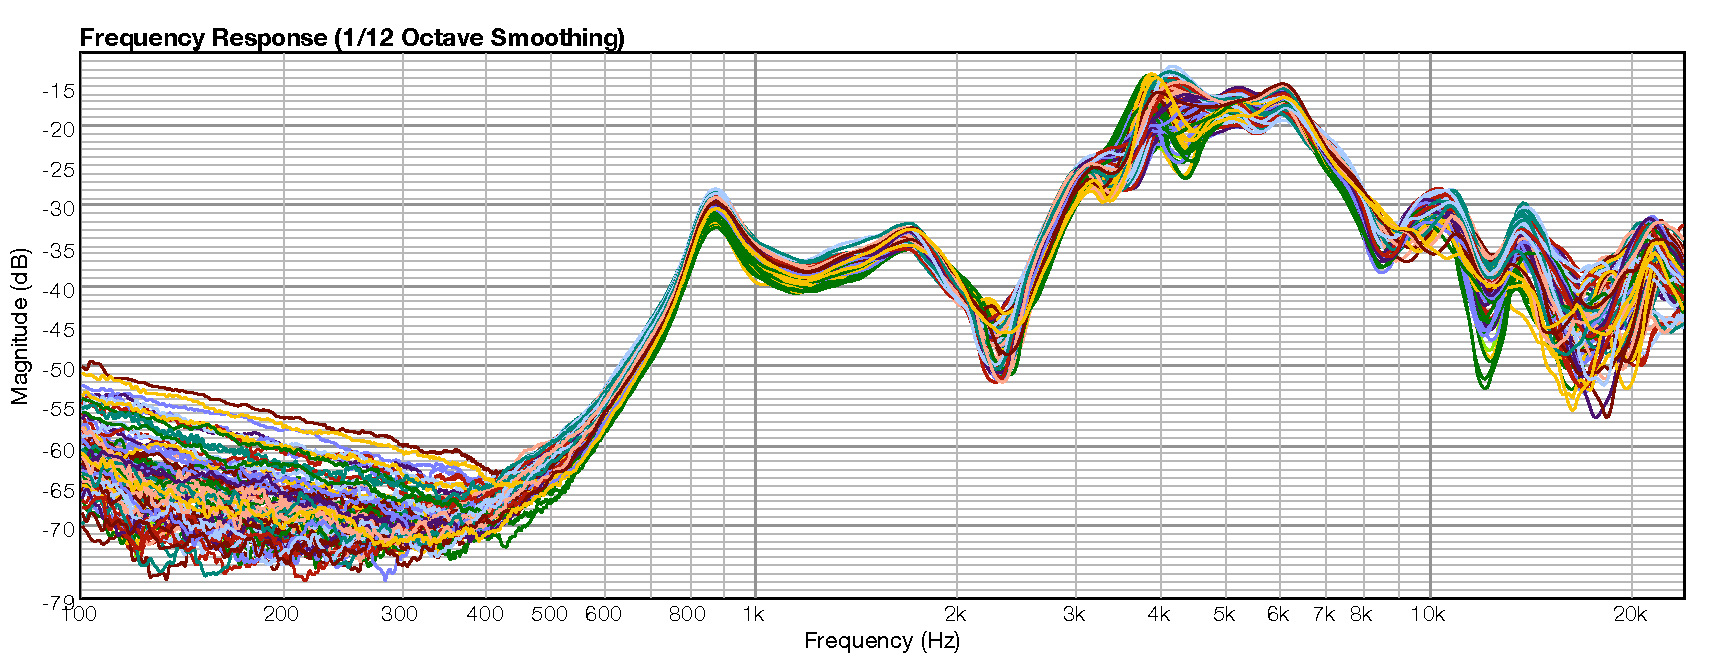
\includegraphics[height=6cm,angle=-90]{shell-all.pdf}
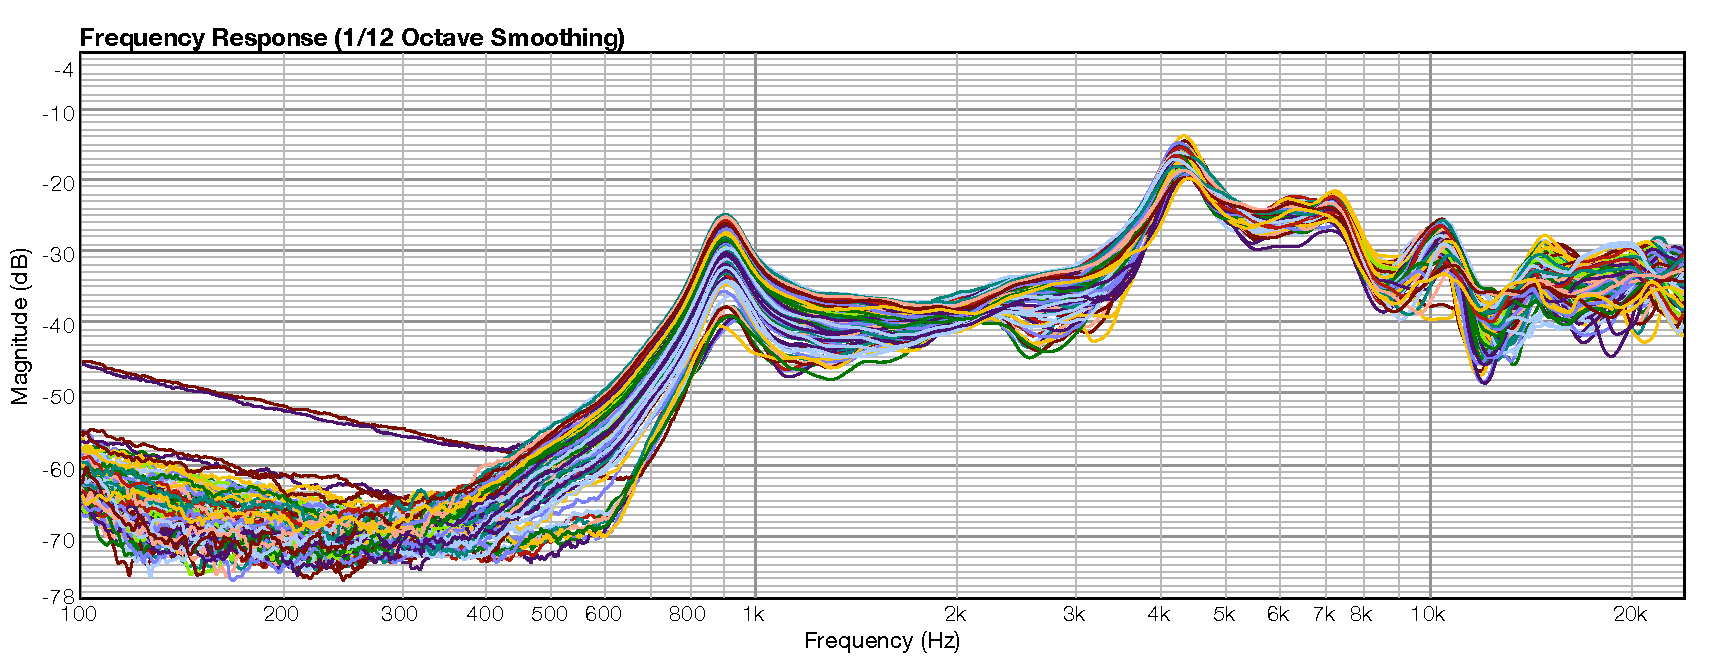
\includegraphics[height=6cm,angle=-90]{noshell-all.pdf}
\end{center}
\caption{Alle m�linger, venstre med kabinet, h�jre uden kabinet}
\label{all}
\end{figure}

% on-axis med og uden kabinet
\begin{figure}
\begin{center}
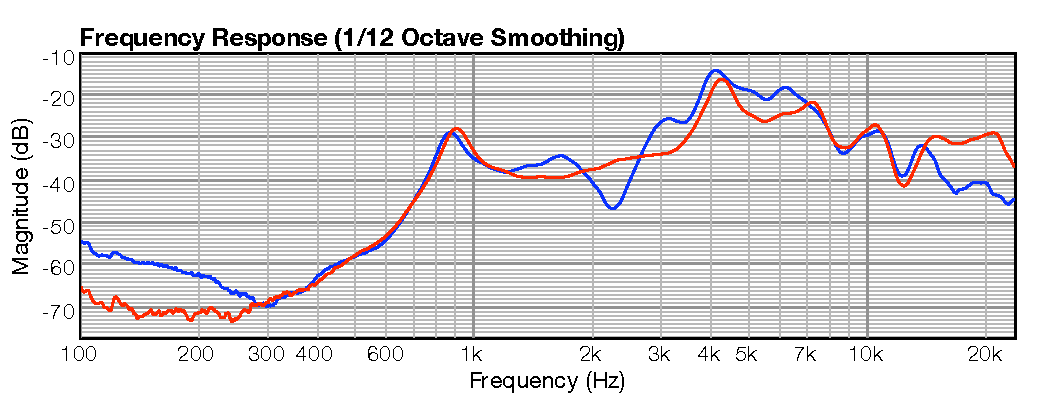
\includegraphics[height=6cm,angle=-90]{onaxis-shell-noshell.pdf}
\end{center}
\caption{On-axis, bl� = med kabinet, r�d = uden kabinet}
\label{onaxis}
\end{figure}

% on-axis med kabinet og s� -40 til 0 horisontalt
% on-axis med kabinet og s� -40 til 0 vertikalt
\begin{figure}
\begin{center}
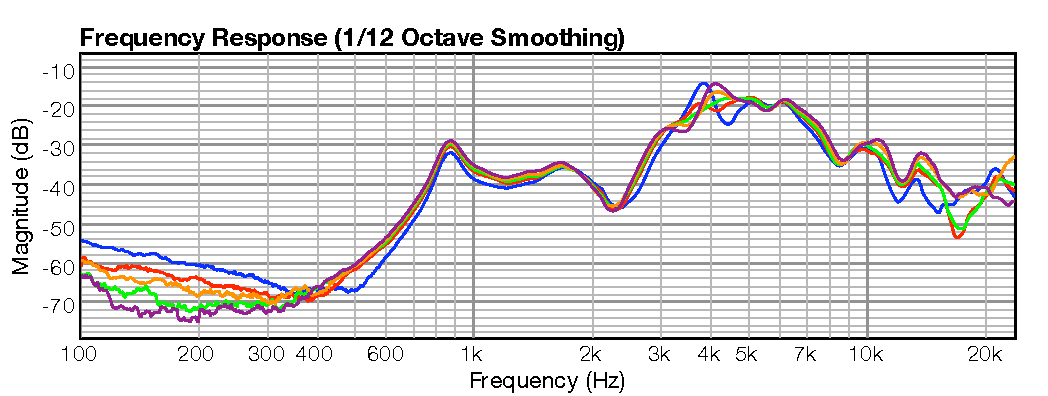
\includegraphics[height=6cm,angle=-90]{minus40to0horizontal.pdf}
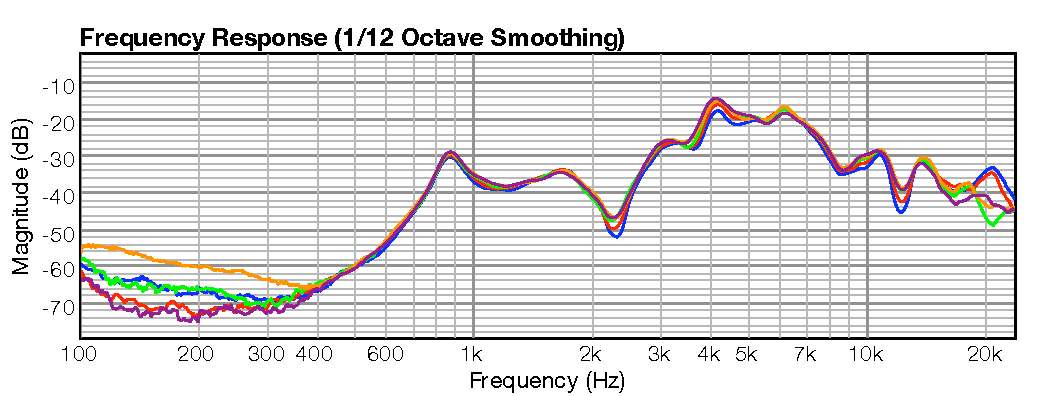
\includegraphics[height=6cm,angle=-90]{minus40to0vertical.pdf}
\end{center}
\caption{venstre horisontal, h�jre vertikal, bl�, r�d, gr�n,orange, lilla = -40, -30, ... , 0}
\label{orto}
\end{figure}



% to meter v�k, b�de hen mod lytteren og v�k fra lytteren
\begin{figure}
\begin{center}
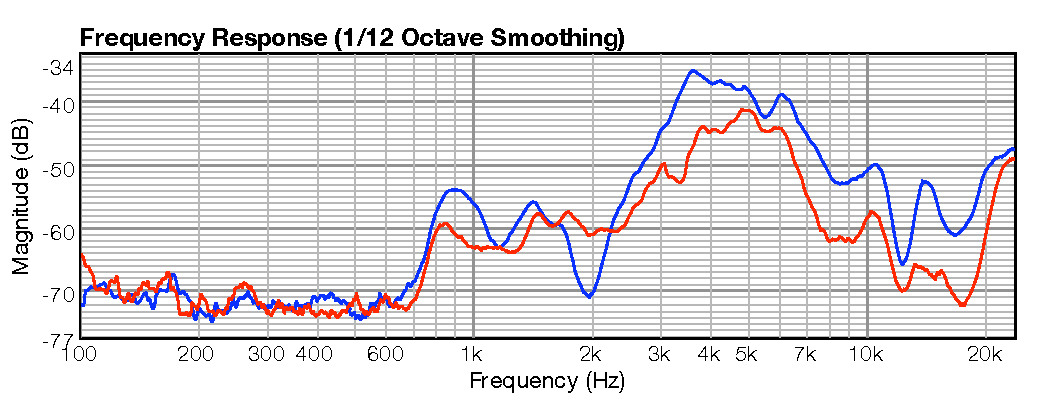
\includegraphics[height=6cm,angle=-90]{2mdist.pdf}
\end{center}
\caption{2 meters afstand, bl� = imod mikrofonen, r�d = v�k fra mikrofonen}
\label{2mdist}
\end{figure}

